
\documentclass[paper=a4, fontsize=11pt]{scrartcl} % A4 paper and 11pt font size

\usepackage[T1]{fontenc} % Use 8-bit encoding that has 256 glyphs
\usepackage{fourier} % Use the Adobe Utopia font for the document - comment this line to return to the LaTeX default
\usepackage[english]{babel} % English language/hyphenation
\usepackage{amsmath,amsfonts,amsthm} % Math packages
\usepackage{graphicx}
\usepackage{float}
\usepackage{subfig}
\usepackage{caption}
\usepackage[section]{placeins}
\usepackage{sectsty} % Allows customizing section commands
\allsectionsfont{\centering \normalfont\scshape} % Make all sections centered, the default font and small caps
\numberwithin{equation}{section} % Number equations within sections (i.e. 1.1, 1.2, 2.1, 2.2 instead of 1, 2, 3, 4)
\numberwithin{figure}{section} % Number figures within sections (i.e. 1.1, 1.2, 2.1, 2.2 instead of 1, 2, 3, 4)
\numberwithin{table}{section} % Number tables within sections (i.e. 1.1, 1.2, 2.1, 2.2 instead of 1, 2, 3, 4)

\setlength\parindent{0pt} % Removes all indentation from paragraphs - comment this line for an assignment with lots of text

%----------------------------------------------------------------------------------------
%	TITLE SECTION
%----------------------------------------------------------------------------------------

\newcommand{\horrule}[1]{\rule{\linewidth}{#1}} % Create horizontal rule command with 1 argument of height

\title{	
\normalfont \normalsize 
\textsc{PH 481 Lab} \\ [25pt] % Your university, school and/or department name(s)
\horrule{2pt} \\[0.5cm] % Thin top horizontal rule
\huge Optics Lab 5\\ % The assignment title
\horrule{2pt} \\[0.5cm] % Thick bottom horizontal rule
}

\author{Harsukh Singh} % Your name

\date{\normalsize \today} % Today's date or a custom date

\begin{document}

\maketitle % Print the title
\section{Overview of Experiment}
\FloatBarrier
This lab explored the process of diffraction with the single, double and many slit aperatures. This process of diffraction is called the Fraunhofer diffraction since the point of observation is very distant from the coherent line source $ R >> D$.  The experimental set up is shown in the figure 1.1, the laser where the laser is aligned to the optical rail (the focus is set at infinity).  The fringe location is y and distance from the screen is D.

\begin{figure}[htb]
\centering
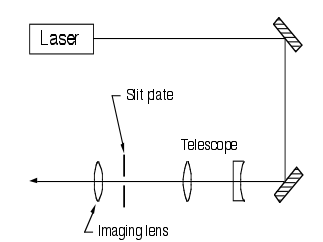
\includegraphics[scale =0.5]{stage}
\caption{Experimental Set-up}
\end{figure}

The zeros of the irradiance (dark fringes) of the single slit can be decribed $bsin(\theta_m) = m \lambda$  where m is an integer. The width of the slit(s) throught the experiment was approximately 0.05 mm and the distance from the screen was approximately 65 cm. The irradiance resulting from the fraunhofer approximation can be described by  $ \frac{I(\beta)}{I(0)} = sinc^2(\beta)$, shown figure 1.2.  The data collected is shown in table 1.1. 
\begin{table}
  \centering 
   \caption{data}
  \begin{tabular}{|l |r| }
    \hline
     fringe 3 & 1.75 cm \\ \hline
     fringe 2 & 1.05 cm \\ \hline
     fringe 1 & 0.5  cm \\  \hline
  \end{tabular}
\end{table}
\begin{figure}[H]
\centering
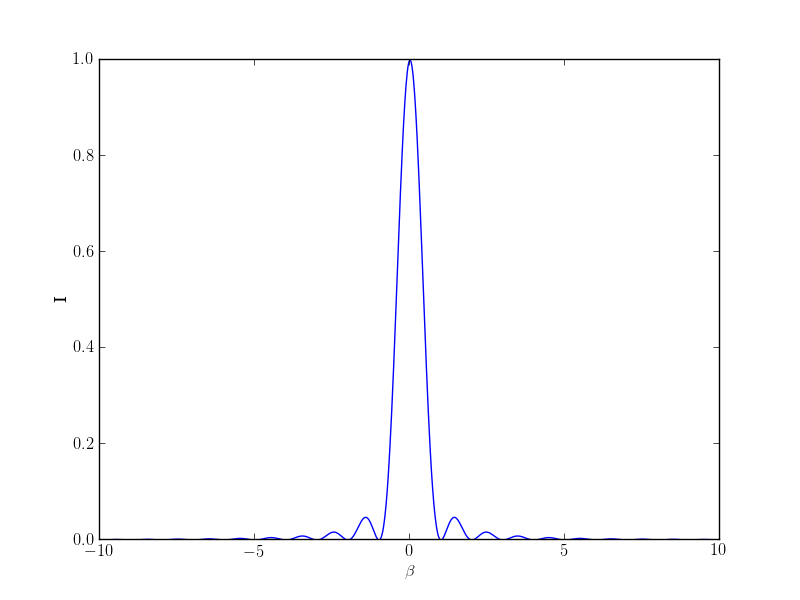
\includegraphics[scale =0.4]{fringes}
\caption{Irradiance}
\end{figure}
We can experimentally find the slit width b by counting the number of fringes at each location knowing that the distance from the center fringe to first so $\theta = tan^{-1}(\frac{y}{D})$. Using the condition for the minimum we find that the slit width is, $ b \approx \frac{m \lambda D}{y} $. Then we find the ratio of $\frac{b}{a} = \frac{m_b}{m_a}$ the derivation is shown below. This can be done by counting the number of principal maxima dark fringes. Thus this gives us the ratio of b to a. The table of the data collected is shown in table 1.2.
\begin{equation}
\frac{bsin(\theta_b)}{asin(\theta_a)} =  \frac{m_by_b}{m_ay_a}
\end{equation}
Using the small angle approximation we arrive at our result.
\begin{figure}[H]
\centering
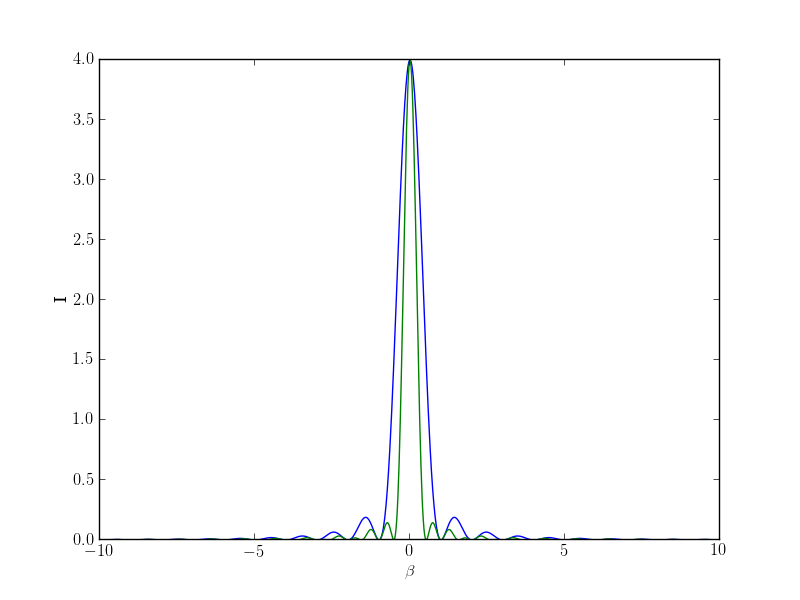
\includegraphics[scale =0.4]{pattern}
\caption{Double slit pattern compared single slit a= 3b}
\end{figure}
\begin{table}
  \centering 
   \caption{data}
  \begin{tabular}{|l |r| }
    \hline
     fringe 3 & 1.00 cm \\ \hline
     fringe 2 & 0.75 cm \\ \hline
     fringe 1 & 0.3  cm \\  \hline
  \end{tabular}
\end{table}
We tested the derivation (eqn (1.1)) and we find that it does work.
\section{Multiple Diffraction Gratings}
In this section we use equation 1.1 and we find the ratios shown in table 2.1. The ratios show the number of principal maxima to second dark fringe (this was the most accurate measurement we could do for this experiment). The number of slits the number of subsidiary maxima.
\begin{table}[H]
  \centering 
   \caption{data}
  \begin{tabular}{|l |r| }
    \hline
     3 slits & $\frac{2}{3}$ \\ \hline
     4 slits & $\frac{2}{4}$ \\ \hline
     10 slits & $\frac{2}{3}$ \\  \hline
  \end{tabular}
\end{table}
These readings have experimental error attached to them because the object was not an exact flat surface as well as measuring every principal maxima between the dark fringes for the single slit may not be entirely accurate due to variance in distance between them. We can describe the pattern of irradiance by the equation,
\begin{equation}
I(\theta) = \frac{I(0)}{N^2} sinc^2(\beta) \left(\frac{sin(N\alpha)}{sin(\alpha)}\right)^2
\end{equation}
We next observed the diffraction pattern from the diffraction slide the screen was $D = 9.5 cm $ and the spacing between the observed pattern was $y =  5.65 cm$. We changed the angle of the slide and observed the spacing between the pattern decrease or increase.  The grating spacing a was determined by 1/N  (N being the number of fringes). \\

We next used the white light and observed the rainbow pattern. 
\section{Fun Experiment}
Here we used a disk with scratches that made a diffraction pattern. The distance between is each grating is 1 mm. 

\section{Conclusion}
%\begin{figure}[htb]
%\centering
%\parbox{5cm}{
%\includegraphics[width=5cm]{figure_1}
%\caption{ Reflection Coefficients}}
%\qquad
%\begin{minipage}{5cm}
%\includegraphics[width=5cm]{figure_2}
%\caption{Transmission Coefficients}
%\end{minipage}
%\end{figure}
%
%\begin{figure}[htb]
%\centering
%\parbox{5cm}{
%\includegraphics[width=5cm]{Epar}
%\caption{Electric Field Parallel to Incident Plane}
%\label{fig:2figsA}}
%\qquad
%\begin{minipage}{5cm}
%\includegraphics[width=5cm]{Eperp}
%\caption{Electric Field Perpendicular to Indicent Plane}
%\label{fig:2figsB}
%\end{minipage}
%%\end{figure}
%
%\section{Experiment 1.1:  Transmittance through Glass}
%\begin{figure}[!ht]
%	\caption{Experimental Set-Up}
%		\begin{center}
%			\includegraphics[scale=0.5]{transmittance}
%		\end{center}
%\end{figure}

%\begin{figure}[!ht]
%	\caption{Experimental Comparison to Theoretical Transmission Coefficients}
%		\begin{center}
%			\includegraphics[scale=0.5]{figure_3}
%		\end{center}
%\end{figure}
%
%\section{Experiment 1.2:  Reflectance from Frosted Glass}
%\begin{figure}[!ht]
%		\begin{center}
%			\includegraphics[scale=0.5]{reflectance}
%		\end{center}
%\caption{Reflectance from Frosted Glass}
%\end{figure}

%\section{Experiment 1.3: Refraction through glass slab}
%\begin{figure}[!ht]
%		\begin{center}
%			\includegraphics[scale=0.5]{GlassLab}
%		\end{center}
%\caption{Measuring the index of refraction through Glass Slab}
%\end{figure}g
% \begin{equation}
%sin(\theta_i -\theta_t) = \frac{l}{\frac{t}{cos(\theta_t)}}
% \end{equation}
% and,
% \begin{equation}
%n_{slab}  = \frac{n_1sin(\theta_1)}{sin(\theta_1-sin^{-1}(\frac{t}{\frac{l}{sin(\theta_i -\theta_t)}}))}
% \end{equation}
% Solving this $n_{slab} = 1.42$  and since most glass has a refractive index of ~1.5 this was pretty close.
% \begin{equation}
%   \begin{tabular}{|l |r| }
%     \hline
%      d(m) & 0.0065561             \\ \hline
%     d^{'} (m) & 0.0064660        \\ \hline
%     d^{''}(m) & 0.006345             \\  \hline
%     d^{'''}(m)& 0.0061452               \\  \hline
%   \end{tabular}
% \end{equation}
% \begin{figure}[htb]
% 	\caption{Fabry-Perot fringes (I vs delta)}
% 		\begin{center}
% 			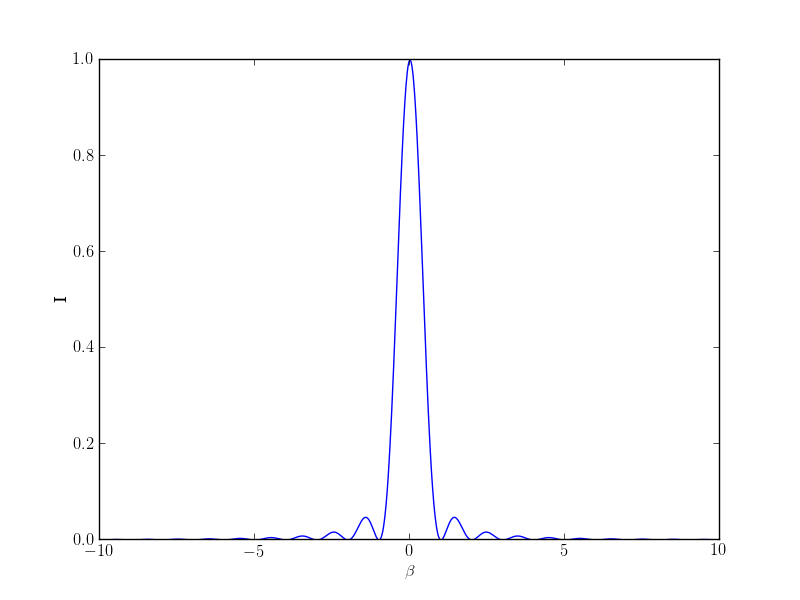
\includegraphics[scale=0.5]{fringes}
% 		\end{center}
% \end{figure}
 \end{document}
